\section{Analisi del dataset}
In questo capitolo viene approfondita la fase di analisi del dataset, organizzata in 2 differenti sezioni che descrivono rispettivamente le attività svolte di esplorazione iniziale e \textit{PCA}. 

Obiettivo della fase iniziale di esplorazione è il controllo riguardante la correttezza del \textit{dataset} caricato e l'analisi delle covariate e le relazioni che intercorrono tra esse. La \textit{PCA} invece, è stata svolta per effettuare un ulteriore studio sulle relazioni tra le covariate ma soprattutto al fine di ridurre la dimensionalità dei dati e contestualmente il loro rumore.

\subsection{Esplorazione del dataset} 
    Inizialmente sono state visualizzate le prime righe del \textit{dataset} (figura \ref{fig:out_head}), per effettuare una prima esplorazione delle variabili e valori presenti. Come è possibile osservare dal grafico, i vini sono descritti solamente da \textit{feature} numeriche. Si può notare inoltre che il \textit{dataframe} presenta esattamente 12 covariate, numero che coincide con quanto indicato nella descrizione del \textit{dataset} \footnote{\href{https://archive.ics.uci.edu/ml/datasets/wine+quality}{UCI Machine Learning: Wine Quality}}. 
    Un ulteriore controllo sulla dimensionalità dei dati ha fornito risultati relativi a numero di colonne (12) e istanze caricate (1599) che hanno trovato anch'essi corrispondenza con quanto dichiarato nella descrizione del dataset. 
    
    \imagespace
    \begin{figure}[h]
        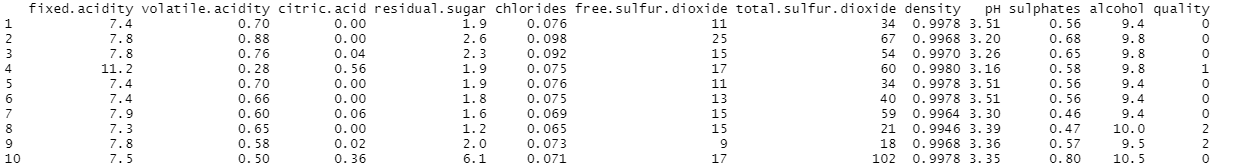
\includegraphics[width=0.95\textwidth]{img/head(wine.data)}
        \centering
        \caption{Prime righe del dataframe}
        \label{fig:out_head}
    \end{figure}
    \imagespace
    
    Successivamente è stata controllata anche la presenza di valori \textit{NA}, che ha dato esito negativo (0 \textit{NA} riscontrati) come già indicato nella descrizione del \textit{dataset}. Questo risultato indica che non è necessaria nessuna politica per la gestione di valori mancanti.
    Infine è stato effettuato un controllo per analizzare la struttura del \textit{dataset} e le tipologie di dati presenti, che ha evidenziato come tutte le covariate fossero di tipo numerico (sia discrete che continue) (figura \ref{fig:out_sapply}). 
    
    I risultati ottenuti da questa esplorazione preliminare ci permettono quindi di affermate che durante il caricamento del dataset non è presente alcun errore, in quanto tutti i valori ottenuti hanno avuto riscontro positivo con quanto dichiarato nella panoramica del dataset.
    
    \begin{figure}[h]
        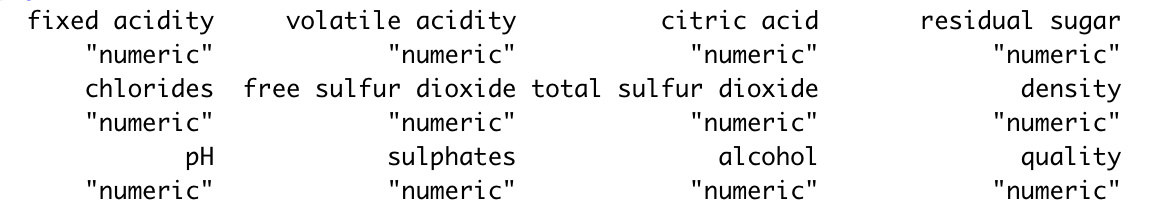
\includegraphics[width=0.9\textwidth]{img/Output_sapply().png}
        \centering
        \caption{Tipi di valori presenti nelle covariate}
        \label{fig:out_sapply}
    \end{figure}
    
    %variabile target e bilanciamento
    Al termine dei controlli riguardanti la correttezza dei dati caricati è stata scelta la covariata \textit{quality} come variabile target, poiché considerata come la più significativa per la predizione (oltre ad essere indicata come tale nella descrizione del dataset). Successivamente è stata controllata attraverso un \textit{barplot} la sua distribuzione dei valori (figura \ref{fig:out_barplot}), dal quale emerge che le istanze siano fortemente sbilanciate. Infatti, la maggior parte dei vini che ha qualità tra i valori 5-6 (82\% delle istanze) e una minoranza che invece presenta qualità bassa (4\%) oppure alta (14\%). 
    Nel dataset inoltre non è presente alcuna istanza con valori 1-2 oppure 9-10. La distribuzione della variabile riflette la distribuzione dei vini nel mondo reale, che vede quelli di qualità media in numero significativamente maggiore rispetto a quello di cattiva e buona qualità. 
    
    \imagespace
    \begin{figure}[!h]
        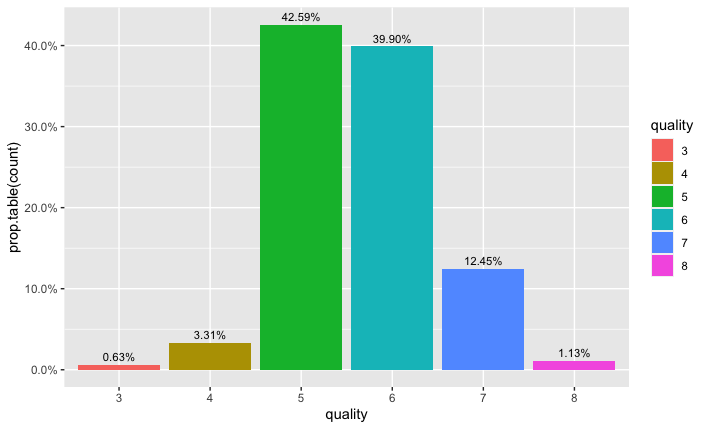
\includegraphics[width=0.9\textwidth]{img/Barplot_quality.png}
        \centering
        \caption{Distribuzione dei valori della feature quality}
        \label{fig:out_barplot}
    \end{figure}

    Dopo aver riscontrato questa distribuzione delle classi abbiamo scelto di ridurre il loro numero, al fine di facilitare i modelli di riconoscimento nella loro classificazione. Per effettuare questa suddivisione, sono state valutate diverse strategie:
    \begin{enumerate}
        \item Ridurre le classi totali da 10 a 5, accoppiando quindi le classi vicine (1-2, 3-4, 5-6, 7-8, 9-10). Il risultato sarebbero quindi state solamente 3 classi (siccome 1-2 e 9-10 non sono presenti), ma le istanze risulterebbero comunque fortemente sbilanciate (14\%, 82\% e 4\% - in ordine di qualità)
        
        \item Trasformare il problema a un problema binario, considerando le classi vini insufficienti (qualità minore di 6) e sufficienti (qualità maggiore o uguale a 6), ottenendo così due classi bilanciate (47\% e 53\% rispettivamente).
        
        \item Focalizzandoci solamente sui valori a disposizione, è possibile identificare 3 diverse classi possibili: 3-5 (qualità bassa oppure \textit{LOW}), 6 (qualità media oppure \textit{MEDIUM}) e 7-8 (qualità alta oppure \textit{HIGH}). Le classi risultano comunque sbilanciate (rispettivamente 46.5\%, 39.9\% e 13.6\%), ma la situazione è migliore rispetto a quanto analizzato nel punto 1. 
    \end{enumerate}
    Si può notare quindi come la soluzione ottimale sia quella presentata nel punto 2, con un problema binario e un bilanciamento quasi perfetto tra le classi. La nostra scelta però è ricaduta sulla terza opzione, poiché:
    \begin{itemize}
        \item Consideravamo la suddivisione binaria un po' meno significativa, dato che la divisione da noi scelta mantiene concettualmente un livello di qualità in più per la catalogazione dei vini.
        \item Ci piaceva l'idea di confrontarci con un problema multiclasse e non solo binario. 
    \end{itemize}
    
    Dopo aver scelto la suddivisione, è stata impostata a categorica la covariata \textit{quality}. La nuova distribuzione di questa feature è illustrata nel \textit{barplot} in figura \ref{fig:out_barplot3}, che fornisce anche informazioni sulla buona riuscita dell'operazione svolta. \'E possibile infatti verificare che i livelli di \textit{quality} sono 3 e non più 6 e che le percentuali cumulate corrispondono. Un ulteriore controllo sulle righe del \textit{dataframe} ha constatato che è stato modificato il numero delle istanze.
    
    \begin{figure}[!h]
        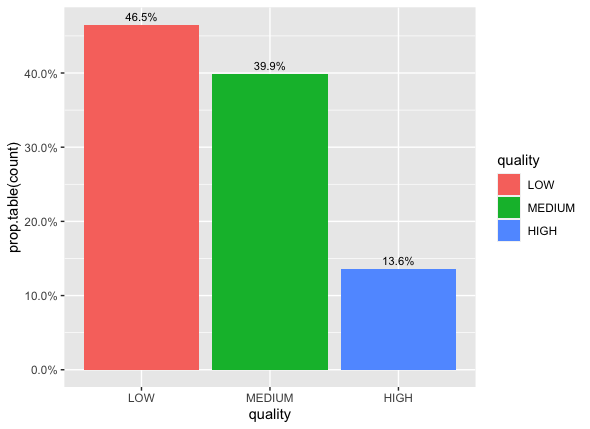
\includegraphics[scale=0.50]{img/Barplot_quality3.png}
        \centering
        \caption{Nuova distribuzione dei valori della feature quality}
        \label{fig:out_barplot3}
    \end{figure}    
    
    Sono stati visualizzati successivamente diversi grafici per l'analisi delle covariate del \textit{dataset}, al fine di comprendere la difficoltà del problema e le studiare relazioni tra le varie \textit{feature}.
    
    Per ogni covariata è stato generato un \textit{boxplot} che mette in relazione i suoi valori con quelli della variabile target. Da questi grafici evince come in realtà nessuna tra le \textit{feature} del \textit{dataset} sia in grado di effettuare una distinzione efficace tra le classi, poiché per tutte le istanze si verifica la sovrapposizione non solo dei "baffi" del grafico, ma anche dei relativi box (dove si concentra la maggior parte dei valori). Inoltre per alcune covariate sono presenti molti \textit{outliers}, che potrebbero causare problemi nella fase successiva di classificazione. 
    Dai grafici si può notare come le covariate \textit{residual.sugar} e \textit{chlorides} siano in assoluto le peggiori, in quanto hanno quasi completamente i box sovrapposti e numerosi \textit{outliers}. Un'altra covariata che presenta un numero notevole di \textit{outliers} è \textit{sulphates}. Le \textit{feature} migliori per la discriminazione (anche se comunque non presentano risultati buoni) sembrano essere \textit{alcohol} e \textit{volatile.acidity}, in quanto le uniche per le quali i box non sono molto sovrapposti, le mediane sono abbastanza lontane per tutte e tre le classi e non presentano molti \textit{outliers}.
    
    \vspace{1.4cm}
    \begin{figure}[h]
        \noindent\makebox[\textwidth]{%
        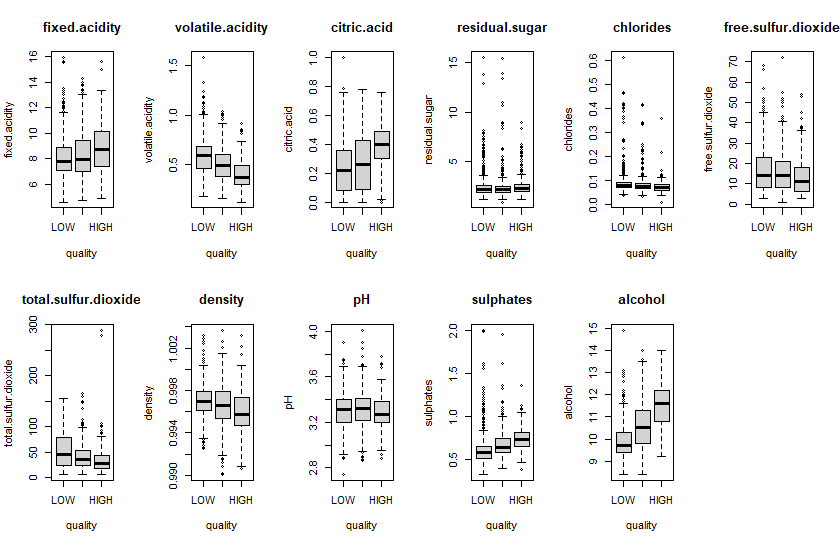
\includegraphics[scale=0.6]{img/boxplot_quality.png}}
        \centering
        \caption{Output boxplot per label}
        \label{fig:out_boxplot_label_2}
    \end{figure}
    
    \newpage
    
    %APPUNTI
    %Dobbiamo mettere in luce nella relazione: presenza di outliers che potrebbero causare qualche problema in fase di classificazione
    %Seconda info: mettendo in relazione i boxplot, vedo se gli intervalli si sovrappongono o meno -> difficoltà a distinguere, quindi quale classe si distingue meglio guardando la covariata xxx ?
    %Maggiorparte dei dati ce l'abbiamo dove c'è il box, però attenzione alle code che si sovrappongono: se si sovrappongono, non è netta la suddivisione
    %Pallini: ouliers - a seconda dell'intervallo di confidena hanno prob bassa di occorrere all'interno della variabile
    
    Anche attraverso la visualizzazione dello \textit{scatterplot} per tutte le covariate (figura \ref{fig:out_scatterplot_matrix}), ci si può rendere conto come in realtà nessuna coppia di esse sia in grado di effettuare una divisione efficace delle classi. Le classi infatti risultano per tutte le combinazioni di molto sovrapposte, e questa condizione è indice del fatto che potrà essere complicato avere una suddivisione efficace delle classi. Le covariate che sembrano suddividere meglio in questo caso le tre classi sembrano essere \textit{free.sulfur.dioxide} e \textit{total.sulfur.dioxide}. Anche osservando la distribuzione delle varie \textit{feature} (figura \ref{fig:out_featureplot}) si può osservare come i valori risultino fortemente sovrapposti e per alcune covariate sono perfettamente sovrapposte anche le distribuzioni stesse.
    
    \vspace{1.2cm}
    \begin{figure}[!h]
        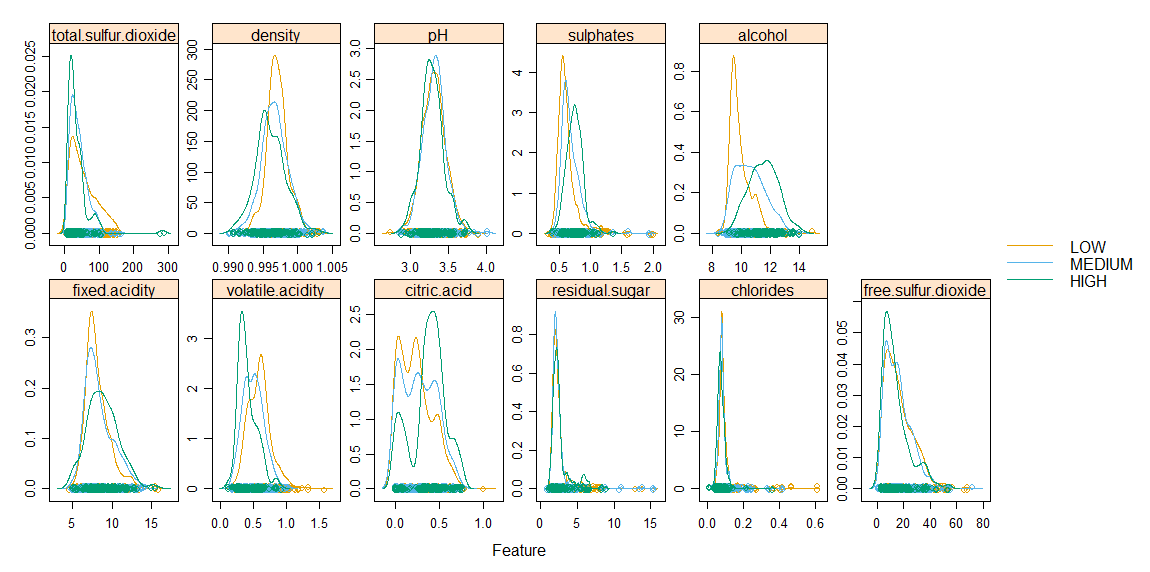
\includegraphics[width=\textwidth]{img/Rplot.png}
        \centering
        \caption{Distribuzione delle variabili}
        \label{fig:out_featureplot}
     \end{figure}   
         
    \newpage
    \begin{figure}[!h]
        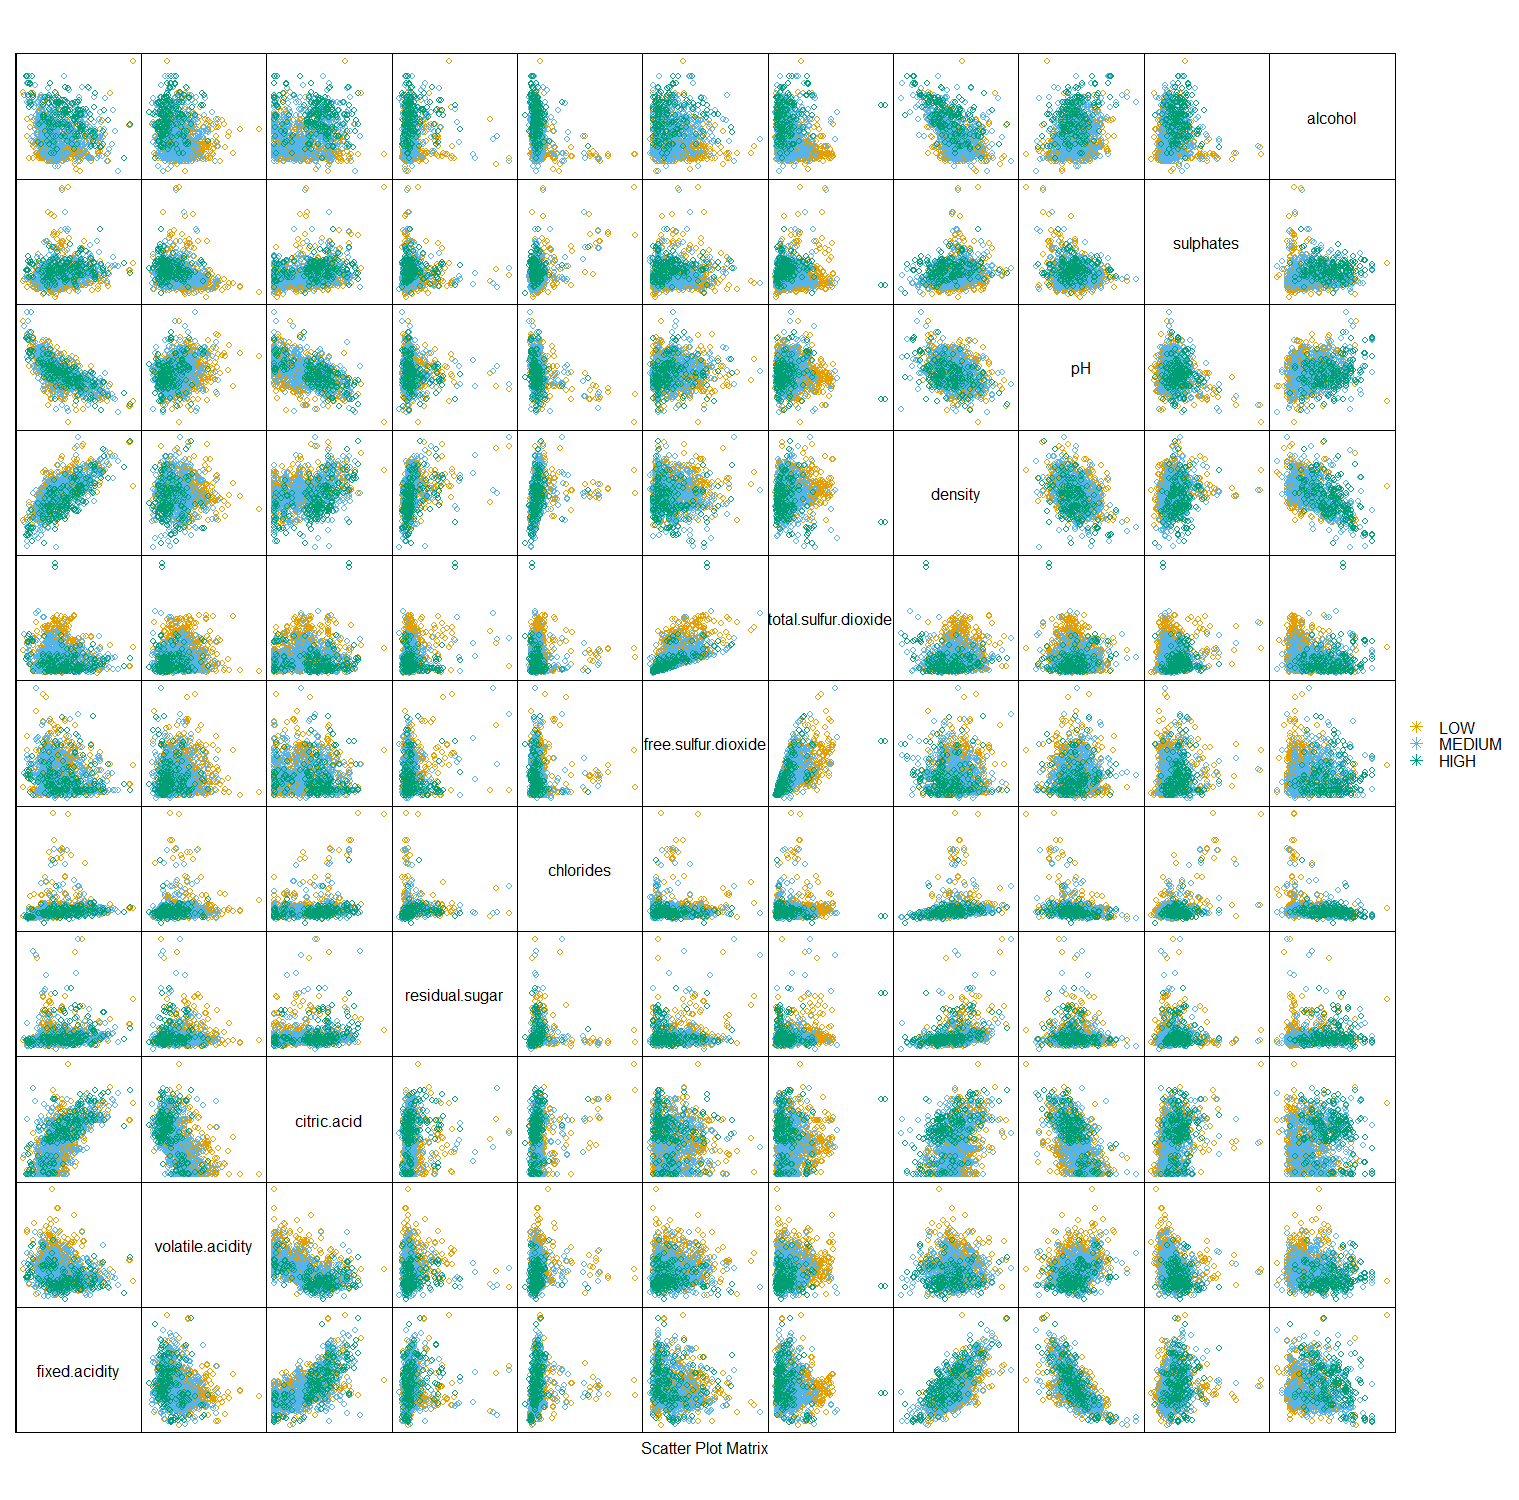
\includegraphics[width=0.9\textwidth]{img/scatterplot_2000.png}
        \centering
        \caption{Scatterplot Matrix}
        \label{fig:out_scatterplot_matrix}
    \end{figure}
    
    \vspace{1cm}
    %TEORIA pallino è l'istanza, serve per capire a coppie di covariate quali siano quelle che dividono meglio una precisa classe
    % Serve per capire quali covariate permettono di discriminare meglio le classi
    
    %\paragraph{Boxplot univariato} a me sembra inutile, risento lab 2 da 58:00 circa
    
    %\paragraph{featurePlot} capire bene (cercando su internet) cosa ci dice. Serve a vedere come si ditribuiscono le covariate
    
%Descrizione del training set: analisi esplorativa del training set (analisi delle covariate e/o PCA)
    % Diagrammi utilizzati per l'esplorazione
    
\subsection{PCA: Principal Component Analysis}
% Note that, the PCA method is particularly useful when the variables within the data set are highly correlated. Correlation indicates that there is redundancy in the data. Due to this redundancy, PCA can be used to reduce the original variables into a smaller number of new variables ( = principal components) explaining most of the variance in the original variables. 
    Al fine di studiare in maniera più approfondita la correlazione tra le variabili e contestualmente provare a ridurre la dimensionalità del dataset e il rumore nei dati, è stata effettuata anche la \textit{Principal Component Analysis}. In un \textit{dataset} non tutti gli attributi sono assolutamente informativi (si può vedere anche dai vari grafici visti finora) ed alcuni possono anche risultare dannosi, aumentando solamente la complessità del modello e rischiando in alcuni casi di confonderlo. Per questi motivi, è stato deciso di utilizzare questo metodo. 
    
    Dopo aver effettuato la \textit{PCA}, è stata osservata la varianza rappresentata da ogni componente. Come si può vedere dagli autovalori presenti nella figura \ref{fig:out_eig}, non sono presenti componenti che singolarmente spiegano una grande quantità di varianza, ma piuttosto la varianza è distribuita in maniera abbastanza omogenea tra diverse le componenti (escluse ovviamente le ultime). 
    
    \begin{figure}[!h]
        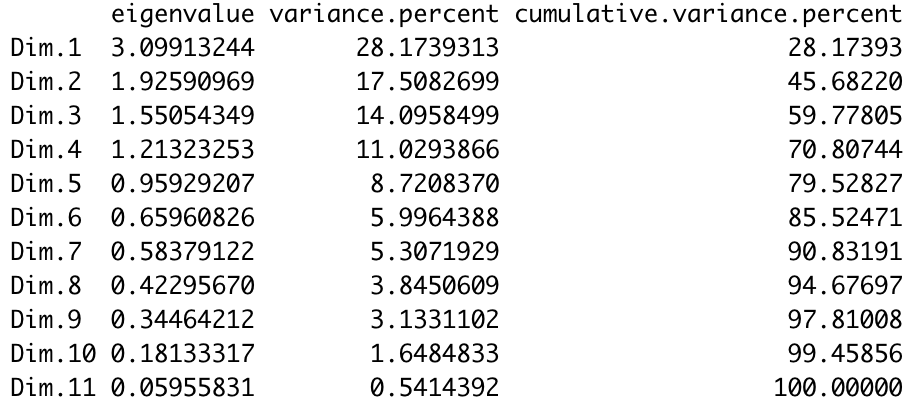
\includegraphics[width=0.7\textwidth]{img/autovalori_pca.png}
        \centering
        \caption{Autovalori PCA}
        \label{fig:out_eig}
    \end{figure} 
    
    Per scegliere quali componenti da mantenere abbiamo deciso di non considerare solamente quelle con autovalori con valore maggiore di 1 ma di scegliere in base alla varianza cumulata, al fine di mantenere un valore di varianza alto. In particolare, è stato deciso di tenere solamente 7 componenti in maniera tale da avere il 90\% della varianza totale. Per effettuare poi le operazioni successive di \textit{train} e \textit{test} è stato considerato il \textit{dataset} prodotto dalla \textit{PCA} nel nuovo spazio di indirizzamento, passando da 11 a 7 dimensioni.
    
    Analizzando le prime due dimensioni della PCA, è possibile effettuare qualche considerazione attraverso alcuni grafici. Osservando il grafico delle variabili (figura \ref{fig:out_pcavar}), si può notare come \textit{sulphates, chlorides e anche residual.sugar} siano le \textit{feature} peggio rappresentate nel nuovo spazio di indirizzamento. Riprendendo le considerazione fatte in precedenza analizzando i boxplot, si può notare come queste siano le variabili che avevamo indicato come le peggiori, sia per sovrapposizione dei valori sia per la presenza di numerosi \textit{outliers}. 
    
    \begin{figure}[!h]
        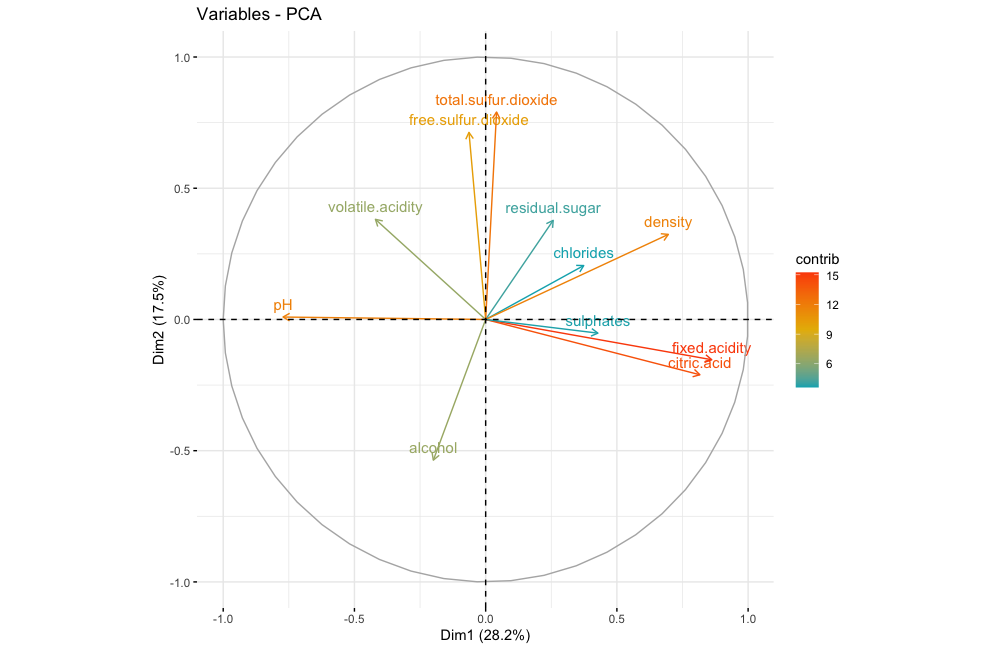
\includegraphics[width=0.9\textwidth]{img/Output_pcavar().png}
        \centering
        \caption{Output fvizpcavar()}
        \label{fig:out_pcavar}
    \end{figure}
    
    Analizzando questo grafico, si possono effettuare anche considerazioni sulla correlazione tra le variabili. Le covariate \textit{fixed.acidity, citric.acid e sulphates} risultano fortemente dipendenti tra loro, come accade per \textit{total.sulfur.dioxide e free.sulfur.dioxide} e anche \textit{chlorides e density}. In generale, la maggior parte delle variabili risulta linearmente dipendente (più o meno fortemente), in quanto le frecce sono tutte concentrate nel quadrante in alto a dx (o nelle sue vicinanze). Le \textit{feature} \textit{alcohol}, \textit{pH} e \textit{volatile.acidity} risultano invece poco correlate rispetto a tutte le altre (soprattutto \textit{alcohol}).

    Un altro grafico sul quale si possono effettuare alcune considerazioni è quello degli \textit{individuals} (figura \ref{fig:out_pcaind}).
    Si può verificare come nel nuovo spazio di rappresentazione (considerando solo le prime due dimensioni), molte istanze non vengano ben rappresentate (colorate di azzurro e verde, concentrate al centro del grafico). Inoltre dal grafico riguardante la classificazione si può osservare che le sole prime due dimensioni non siano necessarie per una suddivisione efficace delle istanze, in quanto tutti gli elementi risultano fortemente sovrapposti. 
    
    Questi risultati ci suggeriscono che anche utilizzando il nuovo spazio di indirizzamento, potremmo avere comunque problemi ad individuare le diverse classi (questo era un risultato atteso, in quanto abbiamo ridotto la varianza e comunque le due dimensioni spiegano solamente il 45\% della varianza totale). Avendo rimosso però una parte di informazioni ridondanti, potremmo avere come beneficio un aumento della precisione dei modelli, nonché una minore complessità degli stessi. 
    
    \vspace{0.6cm}
    \begin{figure}[!h]
        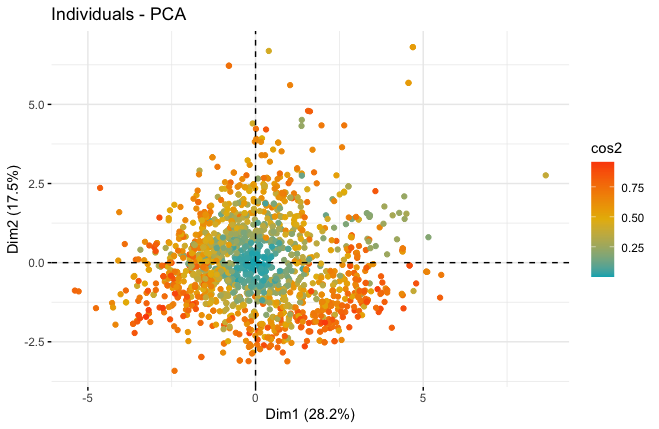
\includegraphics[width=.5\textwidth]{img/individuals_pca_1.png}%
        \qquad
        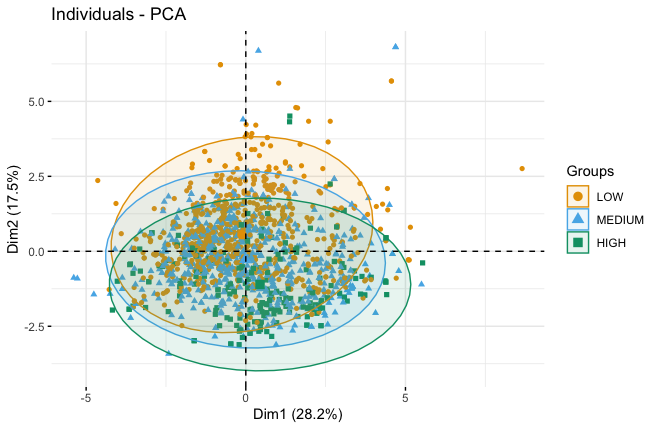
\includegraphics[width=.5\textwidth]{img/individuals_pca_2.png}
        \caption{Individuals PCA}
        \label{fig:out_pcaind}
    \end{figure}
    
    \newpage
